% P1 Task 2 + Task 3 -- academic Beamer deck.
% Build:  pdflatex 2026-07-10-p1-task23-beamer.tex   (run twice for the outline)
% Standard packages only (beamer, booktabs, amsmath, tikz) -- no external theme needed.
\documentclass[10pt,aspectratio=169]{beamer}
\usetheme{Madrid}
\usecolortheme{seahorse}
\usepackage[T1]{fontenc}
\usepackage[utf8]{inputenc}
\usepackage{booktabs}
\usepackage{amsmath,amssymb}
\usepackage{xcolor}
\usepackage{tikz}
\usetikzlibrary{arrows.meta,positioning}

\definecolor{ok}{RGB}{15,110,86}
\definecolor{warn}{RGB}{186,117,23}
\definecolor{bad}{RGB}{160,40,40}
\newcommand{\C}[1]{\texttt{\small #1}}          % inline code (escape _ inside!)
\newcommand{\good}{\textcolor{ok}{\textbf{green}}}
\newcommand{\yes}{\textcolor{ok}{\textbf{yes}}}
\newcommand{\no}{\textcolor{bad}{\textbf{no}}}
\hypersetup{colorlinks=true, urlcolor=blue!60!black, linkcolor=black}   % beamer loads hyperref

\title[P1 Tasks 2 \& 3]{Consolidating \textsc{trx} $\to$ \texttt{tr}:\\
extracting the collision functions and building a $10^{-10}$ fusion oracle}
\subtitle{P1 Task 3 (refactor) and P1 Task 2 (reference capture)}
\author{TASK modernization effort}
\institute[]{Plasma simulation stack --- P1 fusion port, Tasks 1--3 of 10 complete}
\date{2026-07-10}

\begin{document}

\begin{frame}[plain]\titlepage\end{frame}

% ---------------------------------------------------------------------------
\begin{frame}{Outline}
  \tableofcontents
\end{frame}

% ===========================================================================
\section{Context}

\begin{frame}{Where P1 stands}

\textbf{Goal of P1:} make \C{tr} the single canonical transport module by porting bpsi \textsc{trx}'s
multi-reaction fusion physics (\C{model\_pnf}), then archiving \C{trx}/\C{trm} --- \emph{without moving
any existing result}.

\vspace{0.5em}
\begin{columns}[T]
\begin{column}{0.52\textwidth}
\begin{block}{Ledger (10 tasks)}
\small
\begin{tabular}{@{}ll@{}}
\toprule
Task 1 & pre-flight recon $\Rightarrow$ \emph{Option A} \\
\textbf{Task 2} & \textbf{build the $10^{-10}$ reference oracle} \\
\textbf{Task 3} & \textbf{extract collision functions} \\
Tasks 4--6 & fusion data model, \C{libnf}, dispatch \\
Task 7 & validate \C{model\_pnf}=1..4 \\
Tasks 8--10 & species arrays, C-ABI/MCP, archive \\
\bottomrule
\end{tabular}
\end{block}
\end{column}
\begin{column}{0.44\textwidth}
\begin{block}{Option A (owner-decided, Task 1)}
\small
Keep the legacy \C{MDLNF}/\C{SIGMAM} DT path \textbf{exactly as-is}; add \C{model\_pnf} as an
\emph{additive} multi-reaction path, default \textbf{off}.

\medskip
$\Rightarrow$ every ``regression unchanged at $10^{-10}$'' gate becomes trivially satisfiable
\emph{if} the structural work is truly behaviour-preserving.
\end{block}
\end{column}
\end{columns}

\vspace{0.4em}
\begin{alertblock}{This talk}
Task 3 is the structural refactor. Task 2 is the oracle that will judge Tasks 4--7.
Both turned out to rest on plan assumptions that were \emph{false}.
\end{alertblock}
\end{frame}

% ===========================================================================
\section{Task 3 --- extracting the collision functions}

\begin{frame}{Task 3: what the plan said, and what the code actually was}

\begin{center}
\small
\begin{tabular}{@{}p{0.42\textwidth}p{0.52\textwidth}@{}}
\toprule
\textbf{The plan assumed} & \textbf{The code} \\
\midrule
Only \C{trcalc.f90} needs editing
  & \C{COULOG} 12, \C{FTAUE} 8, \C{FTAUI} 11 call sites in \emph{consumer} files, plus \C{HY} 4 ---
    across \textbf{9 files, 10 scopes}. (\C{COULOG} is invoked 3 more times inside \C{trcoll} itself.) \\[0.3em]
They are ordinary functions
  & They are \textbf{bare external} functions; every caller binds them by declaring the name in a
    local \C{REAL(rkind)} list \\[0.3em]
Paste bpsi's \C{trx/trcoll.f90} verbatim
  & bpsi uses \C{PZ(NS\_D)}; kyoshimi \C{tr} defines \textbf{no} \C{NS\_D} $\Rightarrow$ will not compile \\[0.3em]
\C{AMP} and \C{AMM} are the same constant
  & \textcolor{bad}{They are not, any more} --- see next slide \\[0.3em]
Adding \C{trlib} is enough
  & The old external \C{HY} must \emph{also} be deleted, or two live bodies coexist \emph{silently} \\
\bottomrule
\end{tabular}
\end{center}

\vspace{0.3em}
\begin{block}{Consequence}
A ``move three functions'' task became a 12-file change with two genuine numerical hazards.
\end{block}
\end{frame}

% ---------------------------------------------------------------------------
\begin{frame}{Task 3: what moved}

\begin{center}
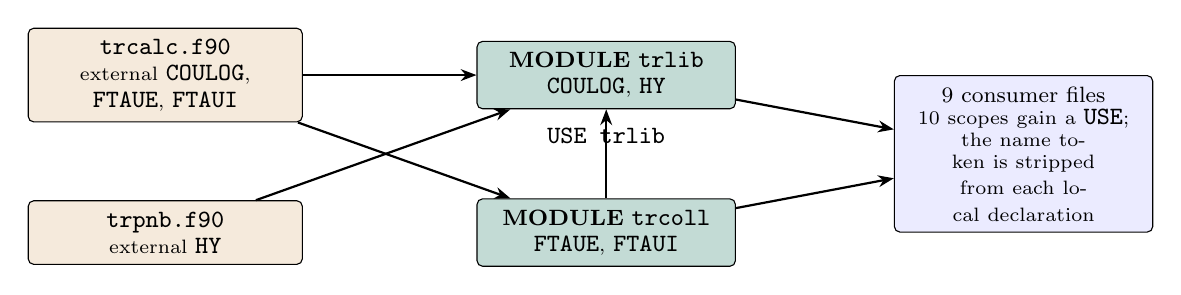
\begin{tikzpicture}[
  box/.style={draw, rounded corners=2pt, align=center, font=\footnotesize, inner sep=4pt, minimum height=8mm},
  ar/.style={-{Stealth[length=2mm]}, thick}
]
  \node[box, fill=warn!15, text width=32mm] (tc) at (0,1.4)
       {\C{trcalc.f90}\\ \scriptsize external \C{COULOG}, \C{FTAUE}, \C{FTAUI}};
  \node[box, fill=warn!15, text width=32mm] (tp) at (0,-0.6)
       {\C{trpnb.f90}\\ \scriptsize external \C{HY}};

  \node[box, fill=ok!25, text width=30mm] (tl) at (5.6,1.4)
       {\textbf{MODULE \C{trlib}}\\ \scriptsize \C{COULOG}, \C{HY}};
  \node[box, fill=ok!25, text width=30mm] (tk) at (5.6,-0.6)
       {\textbf{MODULE \C{trcoll}}\\ \scriptsize \C{FTAUE}, \C{FTAUI}};

  \node[box, fill=blue!8, text width=30mm] (cons) at (10.9,0.4)
       {9 consumer files\\ \scriptsize 10 scopes gain a \C{USE};\\ the name token is stripped\\ from each local declaration};

  \draw[ar] (tc) -- (tl);
  \draw[ar] (tp) -- (tl);
  \draw[ar] (tc) -- (tk);
  \draw[ar] (tk) -- node[above, font=\scriptsize] {\C{USE trlib}} (tl);
  \draw[ar] (tl) -- (cons);
  \draw[ar] (tk) -- (cons);
\end{tikzpicture}
\end{center}

\vspace{-0.3em}
\begin{columns}[T]
\begin{column}{0.48\textwidth}
\begin{block}{Deleted, not merely shadowed}
\C{trcalc.f90}: 1391 $\to$ 1307 lines\\
\C{trpnb.f90}: \phantom{1}553 $\to$ \phantom{1}540 lines
\end{block}
\end{column}
\begin{column}{0.48\textwidth}
\begin{block}{Why a \C{USE} alone is not enough}
A \C{USE}-associated name that is \emph{also} locally typed is a hard \C{gfortran} error ---
so each shared declaration line had to be edited by hand, keeping real externals such as
\C{FTPF}, \C{SIGMAM}, \C{SIGMAB}.
\end{block}
\end{column}
\end{columns}
\end{frame}

% ---------------------------------------------------------------------------
\begin{frame}{Hazard 1: \C{AMP} is no longer \C{AMM}}

bpsi \textsc{trx} takes its constants from \C{bpsd\_constants} (via \C{plcomm}); kyoshimi \C{tr} uses
\C{trcomm\_const} and never touches \C{plcomm}. \C{bpsd} has since moved to the current SI values
(the block is labelled \emph{CODATA 2019} in \C{bpsd\_constants.f90}).

\vspace{0.5em}
\begin{center}
\small
\begin{tabular}{@{}lllr@{}}
\toprule
constant & kyoshimi \C{trcomm\_const} & \C{bpsd\_constants} (CODATA 2019) & rel.\ diff \\
\midrule
\C{AEE}       & \C{1.602176487D-19}  & \C{1.602176634E-19}   & $9.2\times10^{-8}$ \\
\C{AME}       & \C{9.10938215D-31}   & \C{9.1093837015E-31}  & $1.7\times10^{-7}$ \\
\C{AMM}\,/\,\C{AMP} & \C{1.672621637D-27} & \C{1.67262192369E-27} & $1.7\times10^{-7}$ \\
\midrule
\C{PI}, \C{VC}, \C{RMU0}, \C{EPS0} & \multicolumn{2}{l}{bit-identical (verified)} & $0$ \\
\bottomrule
\end{tabular}
\end{center}

\vspace{0.4em}
\begin{block}{Why it matters}
$\mathrm{FTAUI} \propto \sqrt{\mathrm{PAL}\cdot\mathrm{AMM}}$, so a $1.7\times10^{-7}$ constant error
becomes an $\approx 8.6\times10^{-8}$ shift in every ion--ion collision time --- and \C{FTAUI} feeds
the bootstrap current $\mathrm{AJBS}\to\mathrm{AJ}\to\mathrm{QP}$.
That is \textbf{three orders of magnitude above} the $10^{-10}$ regression tolerance.
\end{block}

\begin{exampleblock}{Resolution}
Keep \C{AMM} and \C{PZ(2)}. Take \emph{only} the guard from bpsi. \C{RMU0} is bit-identical despite being
written \C{4.D0*PI*1.D-7} on one side and \C{4.E-7*PI} on the other --- scaling by a power of two commutes
with rounding.
\end{exampleblock}
\end{frame}

% ---------------------------------------------------------------------------
\begin{frame}[fragile]{Hazard 2: the linker will not catch a duplicate}

\C{gfortran} mangles a \emph{module procedure} differently from a \emph{bare external}:

\begin{center}
\begin{minipage}{0.86\textwidth}
\footnotesize
\begin{verbatim}
   MODULE trlib :: HY   ->   ___trlib_MOD_hy      (Mach-O)
   external      HY     ->   _hy_
\end{verbatim}
\end{minipage}
\end{center}

\vspace{0.2em}
These two symbols \textbf{never collide}. Had we added \C{MODULE trlib} while leaving the external
\C{HY} in \C{trpnb.f90}:

\begin{itemize}
  \item callers with \C{USE trlib} bind the module body;
  \item callers without it bind the external body;
  \item the build is \good, the tests pass --- and the two implementations drift apart silently.
\end{itemize}

\vspace{0.3em}
\begin{exampleblock}{Post-condition, checked with \C{nm}}
\footnotesize
Present: \C{\_\_\_trlib\_MOD\_coulog}, \C{\_\_\_trlib\_MOD\_hy},
\C{\_\_\_trcoll\_MOD\_ftaue}, \C{\_\_\_trcoll\_MOD\_ftaui}.\\
Absent: \C{\_coulog\_}, \C{\_ftaue\_}, \C{\_ftaui\_}, \C{\_hy\_}. \quad Single source of truth.
\end{exampleblock}
\end{frame}

% ---------------------------------------------------------------------------
\begin{frame}{Task 3: two commits, exactly one behavioural delta}

\begin{columns}[T]
\begin{column}{0.49\textwidth}
\begin{block}{\C{2baa7948} --- pure move}
Bodies relocated \textbf{character-identical}. Every constant, operator and threshold unchanged.\\[0.3em]
$\Rightarrow$ provably a no-op.
\end{block}
\end{column}
\begin{column}{0.49\textwidth}
\begin{block}{\C{b795c9e6} --- the guard}
Adopt bpsi's
\C{IF(ABS(ANIL).LE.1.D-8) FTAU*=1.D8; RETURN}\\[0.2em]
Replaces an \C{Inf} (divide by $\approx 0$) with a finite value.
\end{block}
\end{column}
\end{columns}

\vspace{0.5em}
\begin{alertblock}{The reviewers disagreed --- so we measured}
One reviewer: \emph{``the guard will fire; \C{tr\_m0904}'s alpha density starts at $\approx 0$; the
$10^{-10}$ gate goes red.''}\\[0.2em]
The inputs say otherwise: \C{tr\_m0904} seeds \C{PN=0.1,0.045,0.045,0.005} and \C{tr\_iter01}
\C{PN=0.7,0.315,0.315,0.035} (units of $10^{20}\,\mathrm{m^{-3}}$) --- \textbf{every} species is 5--6 orders
above the $10^{-8}$ threshold, with the edge pinned by \C{PNS}. The guard cannot fire on a live value.
\end{alertblock}

\vspace{0.2em}
\begin{block}{Where it \emph{does} fire}
\C{tr\_tst2} (\C{NSMAX=2}): the unconditional species-3/4 calls receive $\mathrm{ANT}=\mathrm{ANA}=0$ and
today evaluate to \C{Inf} --- but those results are \emph{dead} in the \C{NSMAX==2} bootstrap branch.
The guard removes a latent NaN that nothing reads.
\end{block}
\end{frame}

% ---------------------------------------------------------------------------
\begin{frame}{Task 3: results}

\begin{center}
\small
\begin{tabular}{@{}llc@{}}
\toprule
Gate & Result & \\
\midrule
\C{make -C tr clean \&\& make -C tr tr2 libtrapi.so} & clean & \yes \\
\C{make -j8 -C tr libtrapi.so} (from clean)     & clean & \yes \\
\C{nm}: module procedures present, no bare externals & as expected & \yes \\
\C{pytest .../test\_equivalence.py --forked}   & 1 passed, 1 xfailed (unchanged) & \yes \\
\C{pytest python/trlib --forked}               & 57 passed, 2 skipped, 1 xfailed, 1 xpassed & \yes \\
\C{tr\_m0904} \C{TR\_REGRESS\_DUMP} dump        & \textbf{byte-identical} to pre-refactor & \yes \\
\bottomrule
\end{tabular}
\end{center}

\vspace{0.5em}
\begin{block}{Covering the case the automated gate does not}
\C{tr\_m0904} is excluded from the \C{pytest} equivalence gate (a documented external-drift issue), yet it is
one of the three baselines Option~A promises bit-for-bit. It was therefore verified \emph{separately}, by
diffing the raw \C{tr\_regress.dat} dump before and after:

\medskip
\centerline{\C{sha256 = 56d09887e679e7ef3c6c54a9cb9ad869} \quad (identical, both runs)}
\end{block}

\vspace{0.2em}
\footnotesize
The 2 skips (missing \C{eqdata}) and the xpass (documented issue \#189) are pre-existing and unchanged.
\end{frame}

% ===========================================================================
\section{Task 2 --- the $10^{-10}$ reference oracle}

\begin{frame}{Task 2: goal, and how the capture is isolated}

\textbf{Goal:} run bpsi \textsc{trx} with \C{model\_pnf=1} (D\,+\,T\,$\to$\,He4\,+\,n) and freeze its output, so
that Tasks 4--7 can validate the kyoshimi port against it at $10^{-10}$.

\vspace{0.4em}
\begin{center}
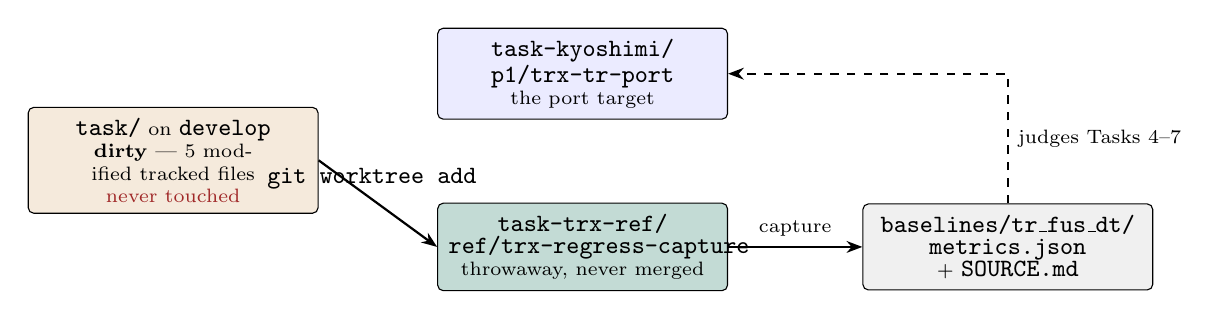
\begin{tikzpicture}[
  box/.style={draw, rounded corners=2pt, align=center, font=\scriptsize, inner sep=4pt, minimum height=9mm, text width=34mm},
  ar/.style={-{Stealth[length=2mm]}, thick}
]
  \node[box, fill=warn!15] (task)  at (0,0)   {\C{task/} on \C{develop}\\ \textbf{dirty} --- 5 modified tracked files\\ \textcolor{bad}{never touched}};
  \node[box, fill=blue!8]  (ky)    at (5.2,1.1) {\C{task-kyoshimi/}\\ \C{p1/trx-tr-port}\\ \scriptsize the port target};
  \node[box, fill=ok!25]   (ref)   at (5.2,-1.1) {\C{task-trx-ref/}\\ \C{ref/trx-regress-capture}\\ \scriptsize throwaway, never merged};
  \node[box, fill=gray!12] (art)   at (10.6,-1.1) {\C{baselines/tr\_fus\_dt/}\\ \C{metrics.json} + \C{SOURCE.md}};

  \draw[ar] (task.east) -- node[above, font=\scriptsize, pos=0.45] {\C{git worktree add}} (ref.west);
  \draw[ar] (ref) -- node[above, font=\scriptsize] {capture} (art);
  \draw[ar, dashed] (art.north) |- node[right, font=\scriptsize, pos=0.25] {judges Tasks 4--7} (ky.east);
\end{tikzpicture}
\end{center}

\vspace{-0.2em}
\begin{block}{Plan Step 1 was unsafe}
It said \C{git checkout -b ref/trx-regress-capture bpsi/develop} \emph{inside} \C{task/} --- a worktree
carrying five uncommitted files. A linked worktree gives the same branch without ever switching the dirty tree.
\end{block}

\vspace{0.2em}
\footnotesize
Captured from bpsi \C{fa9dd493}. The dumper \C{trregress.f90} does not exist in bpsi \textsc{trx} and had to be
ported and wired into \C{trloop.f90}.
\end{frame}

% ---------------------------------------------------------------------------
\begin{frame}{Task 2: reconciling the constants before comparing}

If \textsc{trx} keeps CODATA-2018 while \C{tr} keeps CODATA-2006, the two codes can never agree at
$10^{-10}$ --- \emph{whatever} the fusion model does. So the throwaway capture branch is patched to
kyoshimi's constants:

\vspace{0.4em}
\begin{center}
\small
\begin{tabular}{@{}lp{0.62\textwidth}@{}}
\toprule
site & patch \\
\midrule
\C{trx/trcomm.f90} & rename-import \C{plcomm}'s \C{AEE}/\C{AME}/\C{AMP} out of the way; shadow all three with
                     kyoshimi's values inside \C{trcomm\_parm}. \C{RKEV=AEE*1.D3} follows automatically. \\
\C{trx/libnf.f90}  & \C{PRIVATE :: AEE, AME, AMP} (stop re-exporting bpsd's), and use a local
                     \C{AMP\_kyoshimi} for the DT reduced mass --- \C{libnf} reads \C{AMP} \emph{directly}
                     from \C{bpsd\_constants}, bypassing \C{TRCOMM}. \\
\bottomrule
\end{tabular}
\end{center}

\vspace{0.4em}
\begin{block}{Completeness, verified rather than assumed}
Only \C{trcomm.f90} and \C{libnf.f90} reach those constants outside \C{TRCOMM}. \C{pl}/\C{eq}/\C{bpsd} are
\emph{not} patched: they already use the same values in both trees.
\end{block}

\begin{alertblock}{Contract this imposes on Tasks 4--6}
The ported \C{libnf} must take its constants from kyoshimi \C{TRCOMM}. The plan said
``keep \C{USE bpsd\_constants} as-is'' --- following that would have silently failed Task 7's gate.
\end{alertblock}
\end{frame}

% ---------------------------------------------------------------------------
\begin{frame}{Task 2: is the case even \emph{capable} of a $10^{-10}$ comparison?}

A tolerance is meaningless if the case amplifies floating-point rounding past it. This is measurable, not a
matter of opinion.

\vspace{0.5em}
\begin{block}{The probe}
Perturb one input by a \emph{relative} $10^{-12}$ --- \C{PN(1)}: $0.1 \to 0.1000000000001$ --- rebuild nothing,
re-run, and read the relative change in \textbf{every} entry of \C{metrics.json}.
\[
  A \;=\; \frac{\max_i \;|\Delta y_i / y_i|}{10^{-12}}
  \qquad\Longrightarrow\qquad
  \text{rounding error} \;\approx\; 10^{-16} A
\]
For the comparison to mean anything we need $10^{-16} A \ll 10^{-10}$, i.e. $A \ll 10^{6}$.
\end{block}

\vspace{0.3em}
\begin{exampleblock}{Why this matters here}
The first capture of this oracle was taken at \C{NTMAX=20}, and looked entirely healthy: deterministic,
physical profiles, no \C{NaN}. It was nevertheless \textbf{unusable}.
\end{exampleblock}
\end{frame}

% ---------------------------------------------------------------------------
\begin{frame}{Task 2: the amplification cliff}

\begin{columns}[T]
\begin{column}{0.50\textwidth}
\begin{center}
\small
\begin{tabular}{@{}rrrc@{}}
\toprule
\C{NTMAX} & $A$ & $10^{-16}A$ & $10^{-10}$ usable? \\
\midrule
1  & $0.5$              & $5\times10^{-17}$ & \yes \\
2  & $11$               & $1.1\times10^{-15}$ & \yes \\
\textbf{5}  & $\mathbf{76.5}$ & $\mathbf{7.7\times10^{-15}}$ & \yes \\
10 & $1.1\times10^{2}$  & $1.1\times10^{-14}$ & \yes \\
\midrule
12 & $4.4\times10^{11}$ & $4.4\times10^{-5}$  & \no \\
20 & $2.8\times10^{11}$ & $2.8\times10^{-5}$ & \no \\
\bottomrule
\end{tabular}
\end{center}
\end{column}
\begin{column}{0.47\textwidth}
\begin{block}{Between 10 and 12, a discontinuity}
A $10^{-12}$ input change flips an output by $\approx 28\%$.\\[0.3em]
The profiles stay \emph{physical} there (min $T \approx 4.3\times10^{-2}$ keV, no \C{NaN}) --- so this is not the
solution blowing up. It is a \textbf{discrete branch flip}: an implicit-solve iteration count or an \C{IF}
threshold taking a different path, most plausibly driven by the \C{RIPS=2}$\to$\C{RIPE=3} current ramp.
\end{block}
\end{column}
\end{columns}

\vspace{0.4em}
\begin{alertblock}{At \C{NTMAX=20} the $O(1)$ scalars amplify by $10^{9}$--$10^{11}$}
\C{WPT} $2.6\times10^{9}$, \C{Q0} $1.4\times10^{10}$, \C{BETAP0} $2.8\times10^{11}$.
A $10^{-10}$ comparison there would have been decided by \textbf{rounding, not physics}.
\end{alertblock}

\vspace{-0.1em}
{\scriptsize $A$ is the max over \C{\{WPT, Q0, BETAP0\}} for the scan rows; for the chosen \C{NTMAX=5} it is the
max over \emph{every} entry of \C{metrics.json} (scalars and all 50 profile rows). \C{BETAP0} is the maximiser
throughout.\par}
\end{frame}

% ---------------------------------------------------------------------------
\begin{frame}{Task 2: \C{NTMAX=5}, certified}

\begin{columns}[T]
\begin{column}{0.48\textwidth}
\begin{exampleblock}{Conditioning}
Max amplification over \emph{all} of \C{metrics.json}: $\mathbf{76.5}$\\[0.3em]
Rounding contributes $7.7\times10^{-15}$\\[0.3em]
Margin under $10^{-10}$: $\mathbf{\approx 1.3\times10^{4}\times}$
\end{exampleblock}
\end{column}
\begin{column}{0.48\textwidth}
\begin{exampleblock}{The fusion signal survives}
\C{model\_pnf=1} vs \C{=0}:\\[0.2em]
\C{WPT}\ \ $4.32459894$ vs $4.32363702$\\
\hspace*{1em}$\Rightarrow$ rel $2.2\times10^{-4}$ ($\approx 2\times10^{6}\times$ tol)\\[0.2em]
\C{BETA0} rel $1.6\times10^{-1}$ ($\approx 1.6\times10^{9}\times$ tol)
\end{exampleblock}
\end{column}
\end{columns}

\vspace{0.4em}
\begin{block}{The captured baseline}
\C{NT=5}, \C{NRMAX=50}, \C{NSMAX=4}; 14 scalars + 50 profile rows (\C{RN}, \C{RT}, \C{AJ}, \C{QP}).
Deterministic (repeat capture byte-identical, \C{sha256 1bba5692\ldots}); profiles physical
($T$: $1.017 \to 0.059$ keV core to edge; D and T \emph{densities} bit-identical, their temperatures
differing by $\le 5.5\times10^{-3}$ as the mass ratio $\mathrm{PA}=2$ vs $3$ requires; no \C{NaN}).
\end{block}

\vspace{0.2em}
\begin{block}{Written into the artefact}
\C{SOURCE.md} records the probe, the cliff, and a standing instruction: \emph{if Task 7 ever changes}
\C{NTMAX}\emph{, re-run the probe.}
\end{block}
\end{frame}

% ---------------------------------------------------------------------------
\begin{frame}{Task 2: an argument that had to be retracted}

The first draft of \C{SOURCE.md} justified the constant reconciliation like this:

\begin{quote}
\small\itshape
``Some scalars are strongly sensitive to the constant reconciliation (\C{Q0} $\sim1.4\%$, \C{BETA0}
$\sim35\%$ between OLD and NEW constants) --- this is exactly why the reconciliation is mandatory.''
\end{quote}

\vspace{0.3em}
\begin{alertblock}{The evidence was an artefact}
The constants differ by $\sim 10^{-7}$. A $10^{-7}$ perturbation cannot smoothly produce a $35\%$ swing.
That $35\%$ was simply the \C{NTMAX=20} chaos: at $A \approx 3\times10^{11}$, \emph{any}
$10^{-7}$ perturbation yields $\approx 30\%$.
\end{alertblock}

\vspace{0.3em}
\begin{exampleblock}{The conclusion survives; the reasoning was replaced}
Reconciliation is still mandatory --- but for an arithmetic reason, at the \emph{well-conditioned} operating point:
\[
  \underbrace{1.7\times10^{-7}}_{\text{constant error}} \times \underbrace{76}_{A} \;\approx\; 1.3\times10^{-5}
  \;\ggg\; 10^{-10}.
\]
\end{exampleblock}

\vspace{0.2em}
\centerline{\small\emph{A right answer supported by a wrong measurement is still a defect.}}
\end{frame}

% ===========================================================================
\section{Verification, review, status}

\begin{frame}{What the two independent reviewers caught}

The pre-push gate runs an in-house reviewer and \C{codex} on the same diff. They anchor on different things,
and here they caught different classes:

\vspace{0.4em}
\begin{center}
\small
\begin{tabular}{@{}llp{0.50\textwidth}@{}}
\toprule
sev. & where & finding \\
\midrule
MED & \C{tr/Makefile} & The PIC (\C{libtrapi.so}) build had \textbf{no per-file ordering rules at all}; my
      commit claimed ``\C{make -j} cannot race''. True only for the non-PIC path. \\[0.3em]
MED & \C{tr/trcoll.f90} & The guard returns \emph{before} \C{FTAUE}'s impurity branch, whose denominator uses
      \C{ANEL}, not \C{ANIL}. Broader than ``only fires on a degenerate value''. Deliberate (matches bpsi) --- now
      documented. \\[0.3em]
MED & plan, Task 5 & ``Keep \C{USE bpsd\_constants} as-is'' --- would silently fail Task 7's gate. \\[0.3em]
MED & plan, Task 6 & ``removes the old \C{TRNFDT}/\C{TRNFDHe3}'' --- but Option A keeps the \C{MDLNF SELECT CASE},
      which \emph{calls} them. \\[0.3em]
LOW & plan + \C{SOURCE.md} & I wrote that a $2.2\times10^{-4}$ signal is ``$\sim10^{9}\times$ the tolerance''.
      It is $2.2\times10^{6}\times$. \\
\bottomrule
\end{tabular}
\end{center}

\vspace{0.3em}
\begin{block}{All fixed and re-verified}
\C{make -j8} now builds \C{libtrapi.so} clean from scratch; the plan no longer carries instructions that
Tasks 1--3 disproved.
\end{block}
\end{frame}

% ---------------------------------------------------------------------------
\begin{frame}{Process lessons}

\begin{enumerate}
  \item \textbf{A refactor must be provably a no-op.} Splitting the move from the guard made the single
        behavioural delta bisectable --- and made ``byte-identical'' a checkable claim rather than a hope.

  \item \textbf{Verify the gate before trusting it.} \C{tr\_m0904} is not in the automated equivalence gate.
        Had we relied on \C{pytest} alone, a change to one of the three promised baselines would have been invisible.

  \item \textbf{A tolerance is a property of the \emph{case}, not of the code.} An oracle that amplifies
        $10^{-16}$ into $10^{-5}$ cannot certify anything at $10^{-10}$, no matter how carefully it was captured.

  \item \textbf{Reviewers disagreeing is a signal to measure.} The guard dispute was settled by reading the
        input decks and re-running the dump --- not by picking the more senior-sounding argument.

  \item \textbf{Stale plan text is executable.} Two surviving instructions (\C{USE bpsd\_constants}; delete
        \C{TRNFDT}) would each have broken Task 7 for reasons the same document explained elsewhere.
\end{enumerate}

\vspace{0.3em}
\begin{block}{}
\centering
\small The plan is a hypothesis. Tasks 1--3 falsified five of its assumptions; the document was updated each time.
\end{block}
\end{frame}

% ---------------------------------------------------------------------------
\begin{frame}{Status and next steps}

\begin{columns}[T]
\begin{column}{0.46\textwidth}
\begin{exampleblock}{Delivered (branch \C{p1/trx-tr-port})}
\small
\begin{tabular}{@{}ll@{}}
\C{2baa7948} & extract (pure move) \\
\C{b795c9e6} & vanishing-density guard \\
\C{e8837d92} & the $10^{-10}$ DT oracle \\
\C{a640d818} & PIC \C{-j} ordering fix \\
\C{20ffabbd} & plan brought to as-built \\
\end{tabular}

\medskip
\small P1 ledger: \textbf{3 / 10} tasks complete.
\end{exampleblock}
\end{column}
\begin{column}{0.50\textwidth}
\begin{block}{Next, in dependency order}
\small
\begin{itemize}\itemsep2pt
  \item \textbf{Task 4} --- fusion data model in the split \C{trcomm}, inert (default off)
  \item \textbf{Task 5} --- port \C{libnf} \\ \scriptsize(constants from \C{TRCOMM}, \emph{not} \C{bpsd\_constants})
  \item \textbf{Task 6} --- \C{tr\_pnf} dispatch, \emph{additive}, gated by \C{model\_pnf>0}
  \item \textbf{Task 7} --- validate against the oracle at $10^{-10}$
  \item Tasks 8--10 --- species arrays, C-ABI/MCP, archive \C{trx}/\C{trm}
\end{itemize}
\end{block}
\end{column}
\end{columns}

\vspace{0.3em}
\begin{alertblock}{Open items}
The lab-server checkout sits at \C{c4e0defe} (2026-05-14): 45 commits behind \C{kyoshimi-develop}, and it does
not contain the P0 merge at all. Separately, \C{kyoshimi-develop} has \emph{not} been advanced to the six commits
above --- P1 is incomplete, so that is a deliberate call to make.
\end{alertblock}

\vspace{0.4em}
\centerline{\href{https://github.com/HengyuLi-Ozaki-lab/task/tree/p1/trx-tr-port}{\C{HengyuLi-Ozaki-lab/task}} $\to$ branch \C{p1/trx-tr-port}}
\end{frame}

% ---------------------------------------------------------------------------
\begin{frame}[plain]
\vfill
\centering
{\Large Thank you}\\[1em]
{\small
Task 3: a three-function move that touched nine files and two physical constants.\\
Task 2: an oracle that was healthy, deterministic, physical --- and useless, until it was measured.}
\vfill
\end{frame}

\end{document}
